\prob
{
    Construct the geometric duals of the plane graphs in the next figures.
		    \begin{center}
                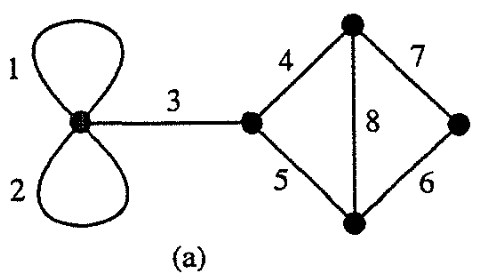
\includegraphics[width=5cm]{Test2/Problem10/Figure1_4.png}
            \end{center}\pn
						
			\begin{center}
                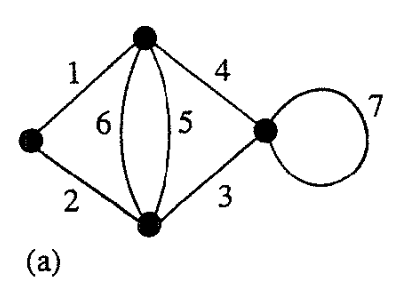
\includegraphics[width=5cm]{Test2/Problem10/Figure1_28.png}
            \end{center}\pn
}
\begin{proof}$\,$\pn
    \begin{figure}[H]
        \begin{center}
        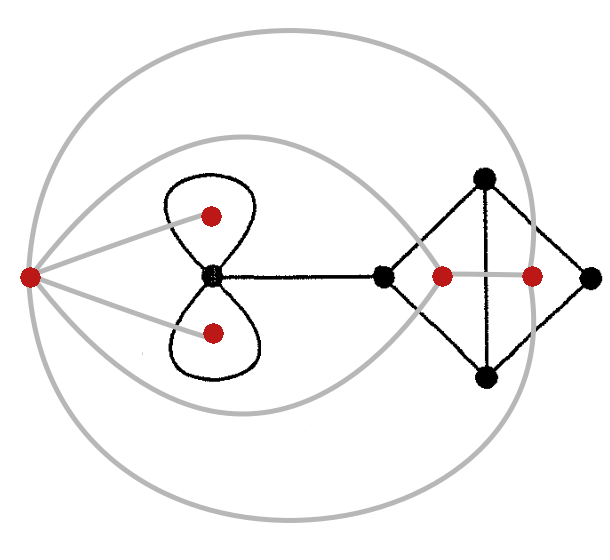
\includegraphics[width=5cm]{Test2/Problem10/Figure1_4_and_its_dual.png}
        \end{center}                            
        \caption{First graph and its dual}
        \label{t2:p9_Figure1_4_and_its_dual.png}                        
    \end{figure}\pn 
    
    \begin{figure}[H]
        \begin{center}
        \includegraphics[width=5cm]{Test2/Problem10/Figure1_4_dual.png}
        \end{center}                            
        \caption{First graph's dual}
        \label{t2:p9_Figure1_4_dual.png}                        
    \end{figure}\pn       
    
    \begin{figure}[H]
        \begin{center}
        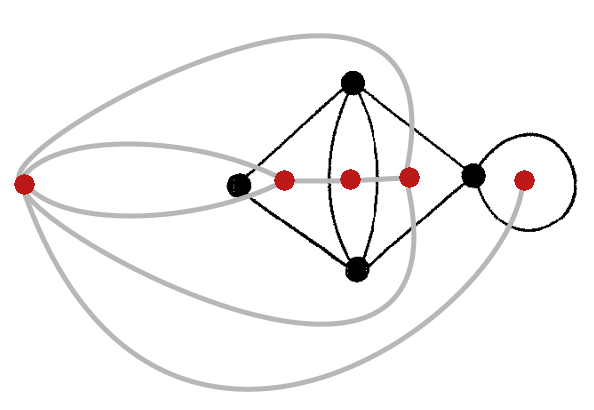
\includegraphics[width=5cm]{Test2/Problem10/Figure1_28_and_its_dual.png}
        \end{center}                            
        \caption{Second graph with its dual}
        \label{t2:p9_Figure1_28_and_its_dual.png}                        
    \end{figure}\pn   
        
    \begin{figure}[H]
        \begin{center}
        \includegraphics[width=5cm]{Test2/Problem10/Figure1_28_dual.png}
        \end{center}                            
        \caption{Second graph's dual}
        \label{t2:p9_Figure1_28_dual.png}                        
    \end{figure}\pn    
\end{proof}